\documentclass{standalone}

\usepackage{tikz}

\begin{document}
	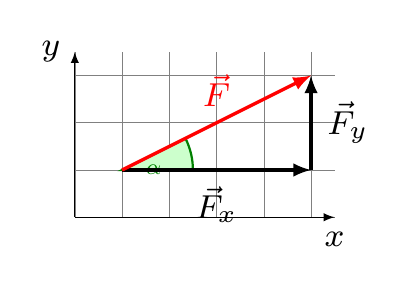
\begin{tikzpicture}
		[
		x=1cm, y=1cm, scale=0.6, font=\footnotesize, >=latex 
		%Voreinstellung für Pfeilspitzen
		]
		
		%Raster im Hintergrund
		\draw[step=1, gray, very thin] (0,0) grid (5.5,3.5);
		
		
		%Länge x Achse
		\draw [-latex] (0,0) -- ++(5.5,0) node[below, scale=1.5] {$x$};
		
		%Länge y Achse
		\draw [-latex] (0,0) -- ++(0,3.5) node[left, scale=1.5] {$y$};
		
		
		%Winkel
		\filldraw[fill=green!20!white, draw=green!50!black, thick] (1,1) -- (2.5,1) arc (0:26.56:1.5) -- cycle node[midway, below, green!50!black] {$\alpha$};		
		
		%Vektor a
		\draw[-latex, very thick] (5,1) -- (5,3) node [midway, right, scale=1.5] {$\vec{F}_y$} node (Fy) {}; 
		%Vektor b
		\draw[-latex, very thick] (1,1) -- (5,1) node [midway, below, scale=1.5] {$\vec{F}_x$} node (Fx) {}; 
%		\draw[dashed] (a.center) -- ++ (3,0) node (c) {};
%		\draw[dashed] (b.center) -- ++ (2,3);
		\draw[very thick, red, -latex] (1,1) -- (Fy.center) node [midway, above, scale=1.5] {$\vec{F}$} node (F) {};
	\end{tikzpicture}
\end{document}